% Канонический TikZ-рисунок варианта 19. Править только здесь.
\long\def\figStereoV19{%
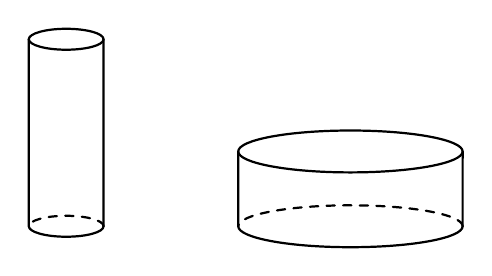
\begin{tikzpicture}[
  scale=0.95,
  line cap=round,
  line join=round
]
  % Первый цилиндр:
  % r_1 = 0.5, h_1 = 2.5
  \coordinate (L1) at (-0.5,0);
  \coordinate (R1) at (0.5,0);

  \draw[thick]
    (0,2.5) ellipse[x radius=0.5,y radius=0.14];

  \draw[thick]
    (L1) -- (-0.5,2.5);

  \draw[thick]
    (R1) -- (0.5,2.5);

  % Передняя и задняя части нижнего основания
  \draw[thick]
    (-0.5,0)
    arc[
      start angle=180,
      end angle=360,
      x radius=0.5,
      y radius=0.14
    ];

  \draw[thick,dashed]
    (0.5,0)
    arc[
      start angle=0,
      end angle=180,
      x radius=0.5,
      y radius=0.14
    ];

  % Второй цилиндр:
  % r_2 = 3r_1 = 1.5,
  % h_2 = h_1/2.5 = 1
  \coordinate (L2) at (2.3,0);
  \coordinate (R2) at (5.3,0);

  \draw[thick]
    (3.8,1)
    ellipse[x radius=1.5,y radius=0.28];

  \draw[thick]
    (L2) -- (2.3,1);

  \draw[thick]
    (R2) -- (5.3,1);

  % Передняя и задняя части нижнего основания
  \draw[thick]
    (2.3,0)
    arc[
      start angle=180,
      end angle=360,
      x radius=1.5,
      y radius=0.28
    ];

  \draw[thick,dashed]
    (5.3,0)
    arc[
      start angle=0,
      end angle=180,
      x radius=1.5,
      y radius=0.28
    ];
\end{tikzpicture}
}
